% ============================================================================
% PLANTILLA PARA AGREGAR NUEVOS EJERCICIOS
% Copia y pega esta plantilla en main.tex donde quieras agregar ejercicios
% ============================================================================

% ----------------------------------------------------------------------------
% EJEMPLO 1: EJERCICIO DE BÚSQUEDA DE RAÍCES
% ----------------------------------------------------------------------------

\subsection{Tu Método de Búsqueda de Raíces}

\begin{exercise}[Título del Ejercicio]
Encuentra la raíz de $f(x) = $ [TU FUNCIÓN] en el intervalo $[a, b]$ usando 
[MÉTODO] con tolerancia $\varepsilon = $ [VALOR].
\end{exercise}

\begin{solution}
\textbf{Paso 1: Verificación de Hipótesis}

Comprobamos las condiciones necesarias...
\begin{align}
    f(a) &= \text{[CÁLCULO]} \\
    f(b) &= \text{[CÁLCULO]}
\end{align}

\textbf{Paso 2: Aplicación del Método}

El método se define como:
\begin{equation}
    x_{n+1} = \text{[FÓRMULA DEL MÉTODO]}
\end{equation}

\textbf{Paso 3: Iteraciones}

\begin{table}[h]
\centering
\caption{Iteraciones de [NOMBRE DEL MÉTODO]}
\begin{tabular}{@{}cccccc@{}}
\toprule
\textbf{$n$} & \textbf{$x_n$} & \textbf{$f(x_n)$} & \textbf{Error Abs.} & \textbf{Error Rel.} \\ 
\midrule
0 & --- & --- & --- & --- \\
1 & --- & --- & --- & --- \\
2 & --- & --- & --- & --- \\
\bottomrule
\end{tabular}
\end{table}

\textbf{Resultado:} $\boxed{x \approx \text{[VALOR]}}$

\end{solution}

% ----------------------------------------------------------------------------
% EJEMPLO 2: EJERCICIO DE INTERPOLACIÓN
% ----------------------------------------------------------------------------

\subsection{Tu Método de Interpolación}

\begin{exercise}[Interpolación de [TIPO]]
Dados los siguientes puntos:
\begin{equation*}
    \begin{array}{c|cccc}
        x & x_0 & x_1 & x_2 & x_3 \\
        \hline
        f(x) & y_0 & y_1 & y_2 & y_3
    \end{array}
\end{equation*}
Construye el polinomio interpolador y evalúa en $x = $ [PUNTO].
\end{exercise}

\begin{solution}
\textbf{Paso 1: Construcción del Polinomio}

Usando [MÉTODO DE INTERPOLACIÓN]:
\begin{equation}
    P_n(x) = \text{[FÓRMULA]}
\end{equation}

\textbf{Paso 2: Evaluación}

\begin{align}
    P_n(\text{[PUNTO]}) &= \text{[DESARROLLO]} \\
                        &= \text{[RESULTADO]}
\end{align}

\textbf{Visualización:}

\begin{center}
\begin{tikzpicture}
    \begin{axis}[
        width=10cm,
        height=7cm,
        xlabel={$x$},
        ylabel={$y$},
        grid=major,
        legend pos=north west,
        domain=0:4,
        samples=100
    ]
    
    % Tu polinomio interpolador
    \addplot[blue, thick] {TU_FUNCION};
    
    % Puntos de datos
    \addplot[only marks, mark=*, red, mark size=3pt] 
        coordinates {(x0,y0) (x1,y1) (x2,y2) (x3,y3)};
    
    \legend{$P_n(x)$, Datos}
    \end{axis}
\end{tikzpicture}
\end{center}

\end{solution}

% ----------------------------------------------------------------------------
% EJEMPLO 3: EJERCICIO DE INTEGRACIÓN NUMÉRICA
% ----------------------------------------------------------------------------

\subsection{Tu Método de Integración}

\begin{exercise}[Regla de [NOMBRE]]
Calcula la integral:
\begin{equation*}
    I = \int_{a}^{b} f(x) \, dx
\end{equation*}
usando [MÉTODO] con $n = $ [NÚMERO] de subintervalos.
\end{exercise}

\begin{solution}
\textbf{Paso 1: Parámetros del Método}

\begin{align}
    a &= \text{[LÍMITE INFERIOR]}, \quad b = \text{[LÍMITE SUPERIOR]} \\
    n &= \text{[NÚMERO DE SUBINTERVALOS]} \\
    h &= \frac{b - a}{n} = \text{[CÁLCULO]}
\end{align}

\textbf{Paso 2: Puntos de Evaluación}

\begin{table}[h]
\centering
\caption{Evaluaciones de la Función}
\begin{tabular}{@{}ccccc@{}}
\toprule
\textbf{$i$} & \textbf{$x_i$} & \textbf{$f(x_i)$} & \textbf{Coeficiente} \\ 
\midrule
0 & --- & --- & --- \\
1 & --- & --- & --- \\
\vdots & \vdots & \vdots & \vdots \\
n & --- & --- & --- \\
\bottomrule
\end{tabular}
\end{table}

\textbf{Paso 3: Aplicación de la Fórmula}

\begin{align}
    I &\approx \text{[FÓRMULA DE INTEGRACIÓN]} \\
      &= \text{[DESARROLLO]} \\
      &= \text{[RESULTADO]}
\end{align}

\textbf{Análisis de Error:}

Error teórico: $E = \ord(h^\text{[ORDEN]})$

\textbf{Resultado:} $\boxed{I \approx \text{[VALOR]}}$

\end{solution}

% ----------------------------------------------------------------------------
% EJEMPLO 4: EJERCICIO DE ECUACIONES DIFERENCIALES
% ----------------------------------------------------------------------------

\subsection{Tu Método para EDOs}

\begin{exercise}[Problema de Valor Inicial]
Resuelve el PVI:
\begin{equation*}
    \frac{dy}{dx} = f(x, y), \quad y(x_0) = y_0
\end{equation*}
en el intervalo $[x_0, x_f]$ con paso $h = $ [VALOR] usando [MÉTODO].
\end{exercise}

\begin{solution}
\textbf{Paso 1: Formulación del Método}

Para $y' = f(x, y)$, el método [NOMBRE] es:
\begin{equation}
    y_{n+1} = \text{[FÓRMULA ITERATIVA]}
\end{equation}

\textbf{Paso 2: Iteraciones}

\begin{table}[h]
\centering
\caption{Solución Numérica de la EDO}
\begin{tabular}{@{}ccccc@{}}
\toprule
\textbf{$n$} & \textbf{$x_n$} & \textbf{$y_n$} & \textbf{$y_{\text{exacta}}$} & \textbf{Error} \\ 
\midrule
0 & --- & --- & --- & --- \\
1 & --- & --- & --- & --- \\
\vdots & \vdots & \vdots & \vdots & \vdots \\
N & --- & --- & --- & --- \\
\bottomrule
\end{tabular}
\end{table}

\textbf{Visualización Comparativa:}

\begin{center}
\begin{tikzpicture}
    \begin{axis}[
        width=11cm,
        height=7cm,
        xlabel={$x$},
        ylabel={$y$},
        grid=major,
        legend pos=north east,
        domain=0:2,
        samples=100
    ]
    
    % Solución analítica (si existe)
    \addplot[red, thick] {SOLUCION_EXACTA};
    
    % Solución numérica
    \addplot[blue, thick, mark=*, mark size=2pt] 
        coordinates {(x0,y0) (x1,y1) ... (xn,yn)};
    
    \legend{Solución exacta, [MÉTODO]}
    \end{axis}
\end{tikzpicture}
\end{center}

\end{solution}

% ----------------------------------------------------------------------------
% EJEMPLO 5: SISTEMA DE ECUACIONES LINEALES
% ----------------------------------------------------------------------------

\subsection{Tu Método para Sistemas Lineales}

\begin{exercise}[Sistema $n \times n$]
Resuelve el sistema de ecuaciones:
\begin{equation*}
    \matr{A}\vect{x} = \vect{b}
\end{equation*}
donde:
\begin{equation*}
    \matr{A} = \begin{bmatrix}
        a_{11} & a_{12} & \cdots & a_{1n} \\
        a_{21} & a_{22} & \cdots & a_{2n} \\
        \vdots & \vdots & \ddots & \vdots \\
        a_{n1} & a_{n2} & \cdots & a_{nn}
    \end{bmatrix}, \quad
    \vect{b} = \begin{bmatrix}
        b_1 \\ b_2 \\ \vdots \\ b_n
    \end{bmatrix}
\end{equation*}
\end{exercise}

\begin{solution}
\textbf{Paso 1: Matriz Aumentada}

\begin{equation}
    [\matr{A} | \vect{b}] = \left[\begin{array}{cccc|c}
        a_{11} & a_{12} & \cdots & a_{1n} & b_1 \\
        a_{21} & a_{22} & \cdots & a_{2n} & b_2 \\
        \vdots & \vdots & \ddots & \vdots & \vdots \\
        a_{n1} & a_{n2} & \cdots & a_{nn} & b_n
    \end{array}\right]
\end{equation}

\textbf{Paso 2: Aplicación del Método [NOMBRE]}

\textit{[Describe los pasos del método: eliminación, sustitución, iteración, etc.]}

Después de la transformación:
\begin{equation}
    \text{[FORMA REDUCIDA DE LA MATRIZ]}
\end{equation}

\textbf{Paso 3: Solución}

\begin{equation}
    \vect{x} = \begin{bmatrix}
        x_1 \\ x_2 \\ \vdots \\ x_n
    \end{bmatrix} = \begin{bmatrix}
        \text{[VALOR]} \\ \text{[VALOR]} \\ \vdots \\ \text{[VALOR]}
    \end{bmatrix}
\end{equation}

\textbf{Verificación:}

\begin{align}
    \matr{A}\vect{x} &= \text{[PRODUCTO MATRIZ-VECTOR]} \\
                     &= \vect{b} \quad \checkmark
\end{align}

\end{solution}

% ----------------------------------------------------------------------------
% EJEMPLO 6: ALGORITMO EN PSEUDOCÓDIGO
% ----------------------------------------------------------------------------

\subsection{Algoritmo de [Tu Método]}

\begin{algorithm}[H]
\caption{[Nombre del Algoritmo]}
\KwIn{[Parámetros de entrada]}
\KwOut{[Resultado esperado]}

\textbf{Inicialización:} \\
$\text{variable} \leftarrow \text{valor inicial}$\;

\While{condición de continuación}{
    \textbf{Paso iterativo:} \\
    $\text{cálculo}_1 \leftarrow \text{fórmula}_1$\;
    $\text{cálculo}_2 \leftarrow \text{fórmula}_2$\;
    
    \If{condición de verificación}{
        \Return{resultado}\;
    }
    
    $\text{actualización de variables}$\;
    $\text{contador} \leftarrow \text{contador} + 1$\;
}

\Return{resultado final}\;
\end{algorithm}

% ----------------------------------------------------------------------------
% PLANTILLA DE GRÁFICO PERSONALIZADO
% ----------------------------------------------------------------------------

% Gráfico básico de función
\begin{center}
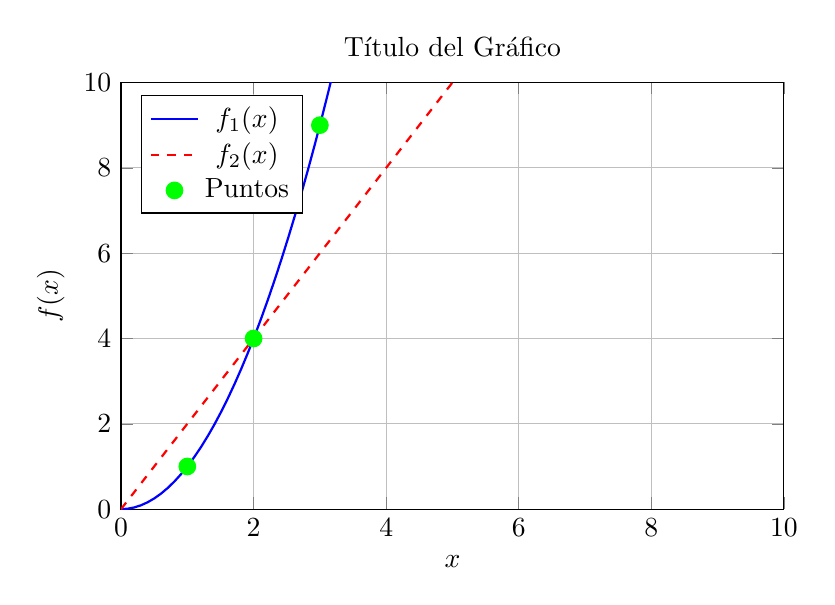
\begin{tikzpicture}
    \begin{axis}[
        width=10cm,
        height=7cm,
        xlabel={$x$},
        ylabel={$f(x)$},
        title={Título del Gráfico},
        grid=major,
        legend pos=north west,
        domain=0:10,
        samples=100,
        xmin=0, xmax=10,
        ymin=0, ymax=10
    ]
    
    % Función 1
    \addplot[blue, thick] {x^2};
    
    % Función 2
    \addplot[red, dashed, thick] {2*x};
    
    % Puntos específicos
    \addplot[only marks, mark=*, green, mark size=3pt] 
        coordinates {(1,1) (2,4) (3,9)};
    
    \legend{$f_1(x)$, $f_2(x)$, Puntos}
    \end{axis}
\end{tikzpicture}
\end{center}

% Gráfico de error (escala logarítmica)
\begin{center}
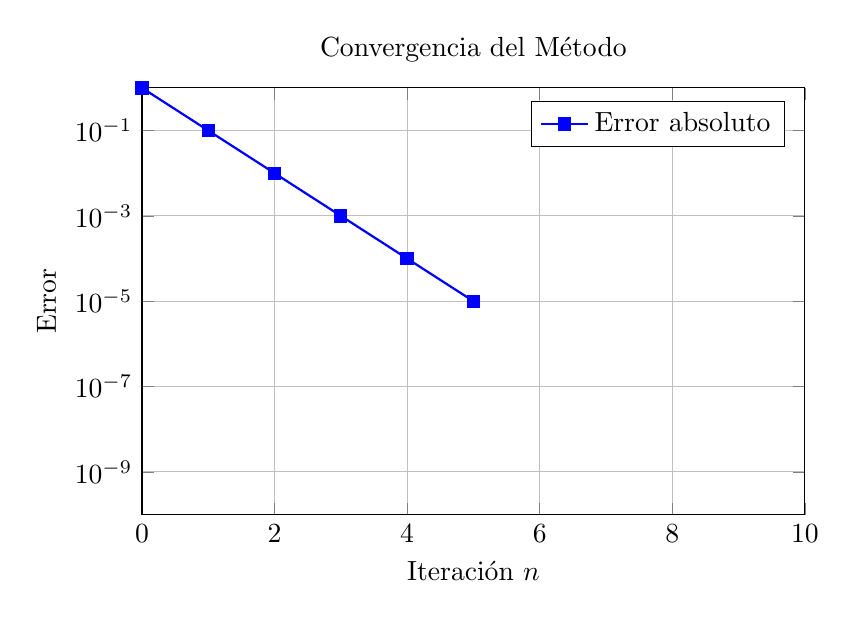
\begin{tikzpicture}
    \begin{axis}[
        width=10cm,
        height=7cm,
        xlabel={Iteración $n$},
        ylabel={Error},
        title={Convergencia del Método},
        grid=major,
        legend pos=north east,
        ymode=log,  % Escala logarítmica en Y
        xmin=0, xmax=10,
        ymin=1e-10, ymax=1
    ]
    
    \addplot[blue, thick, mark=square*] 
        coordinates {(0,1) (1,0.1) (2,0.01) (3,0.001) (4,1e-4) (5,1e-5)};
    
    \legend{Error absoluto}
    \end{axis}
\end{tikzpicture}
\end{center}

% ----------------------------------------------------------------------------
% PLANTILLA DE TABLA PROFESIONAL
% ----------------------------------------------------------------------------

\begin{table}[h]
\centering
\caption{Descripción de la Tabla}
\label{tab:mi_tabla}
\begin{tabular}{@{}lcccc@{}}
\toprule
\textbf{Columna 1} & \textbf{Col 2} & \textbf{Col 3} & \textbf{Col 4} & \textbf{Col 5} \\ 
\midrule
Fila 1 & dato & dato & dato & dato \\
Fila 2 & dato & dato & dato & dato \\
Fila 3 & dato & dato & dato & dato \\
\midrule
\textbf{Total/Promedio} & --- & --- & --- & --- \\
\bottomrule
\end{tabular}
\end{table}

% Referencia a tabla: ver Tabla~\ref{tab:mi_tabla}

% ----------------------------------------------------------------------------
% NOTAS Y OBSERVACIONES IMPORTANTES
% ----------------------------------------------------------------------------

\begin{note}
Usa este entorno para agregar notas importantes o aclaraciones sobre el método.
\end{note}

\begin{remark}
Las observaciones proporcionan insights adicionales sobre el comportamiento del método,
convergencia, estabilidad, o aplicaciones prácticas.
\end{remark}

% ----------------------------------------------------------------------------
% FIN DE PLANTILLA
% ============================================================================
